% !TEX root =  ../supplementary.tex
\section{A Joint Model for the Longitudinal PSA, and Time to Gleason Upgrading}
\label{sec:jm_framework}

Let $T_i^*$ denote the true time of upgrading (increase in biopsy Gleason grade group from~1 to 2 or higher) for the ${i\mbox{-th}}$ patient included in PRIAS. Since biopsies are conducted periodically, $T_i^*$ is observed with interval censoring ${l_i < T_i^* \leq r_i}$. When upgrading is observed for the patient at his latest biopsy time $r_i$, then $l_i$ denotes the time of the second latest biopsy. Otherwise, $l_i$ denotes the time of the latest biopsy and ${r_i=\infty}$. Let $\boldsymbol{y}_{i}$ denote his observed PSA longitudinal measurements. The observed data of all $n$ patients is denoted by ${\mathcal{A}_n = \{l_i, r_i, \boldsymbol{y}_{i}; i = 1, \ldots, n\}}$.

\begin{figure}
\centerline{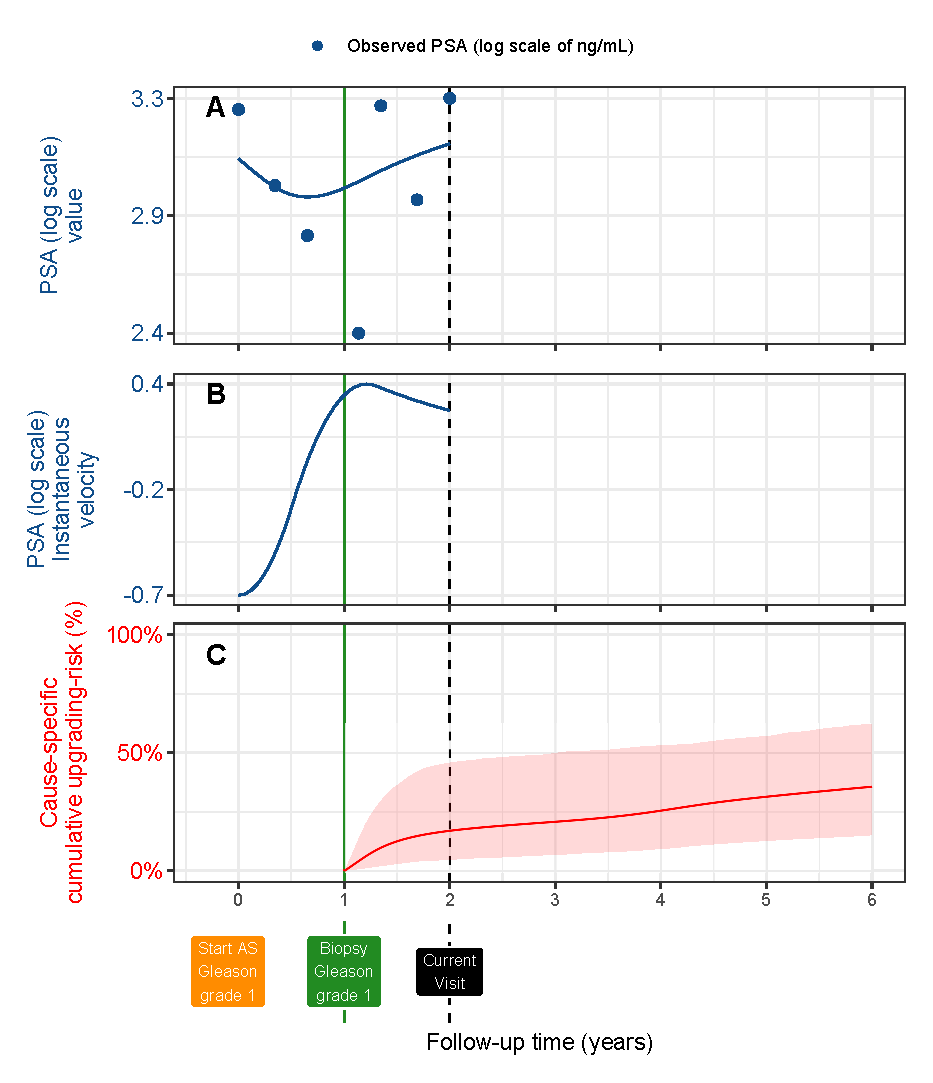
\includegraphics[width=\columnwidth]{images/jmExplanationPlot_113.eps}}
\caption{\textbf{Illustration of the joint model on a real PRIAS dataset patient}. \textbf{Panel~A:} Observed (blue dots) and fitted PSA (solid blue line) measurements, log-transformed. \textbf{Panel~B:} Estimated instantaneous velocity of PSA (log-transformed). \textbf{Panel~C}: Predicted cumulative-risk of upgrading (95\% credible interval shaded). Upgrading is defined as an increase in Gleason grade group \citep{epsteinGG2014} from grade group~1 to 2 or higher. This risk of upgrading is available starting from the time of the latest negative biopsy (vertical green line at year 1 of follow-up). The joint model estimated it by combining the fitted PSA value and velocity (both on the log scale of PSA) and time of the latest negative biopsy. Black dashed line at year 4 denotes the time of current visit.}
\label{fig:jmExplanationPlot_113}
\end{figure}

In our joint model, the patient-specific PSA measurements over time are modeled using a linear mixed effects sub-model. It is given by (see Panel~A, Figure~\ref{fig:jmExplanationPlot_113}):
\begin{equation}
\label{eq:long_model_psa}
\begin{split}
    \log_2 \big\{y_{i}(t) + 1\big\} &= m_{i}(t) + \varepsilon_{i}(t),\\
    m_{i}(t) &= \beta_{0} + b_{0i} + \sum_{k=1}^4 (\beta_{k} + b_{ki})  B_k\Big(\frac{t-2}{2},\frac{\mathcal{K}-2}{2}\Big) + \beta_{5} \mbox{age}_i,
    \end{split}
\end{equation}
where, $m_{i}(t)$ denotes the measurement error free value of $\log_2 (\mbox{PSA} + 1)$ transformed \citep{pearson1994mixed,lin2000latent} measurements at time $t$. We model it non-linearly over time using B-splines \citep{de1978practical}. To this end, our B-spline basis function ${B_k\{(t-2)/2,(\mathcal{K}-2)/2\}}$ has three internal knots at $\mathcal{K} = \{0.5, 1.3, 3\}$ years, which are the three quartiles of the observed follow-up times. The boundary knots of the spline are at 0 and 6.3 years (95-th percentile of the observed follow-up times). We mean centered (mean 2 years) and standardized (standard deviation 2 years) the follow-up time $t$ and the knots of the B-spline $\mathcal{K}$ during parameter estimation for better convergence. The fixed effect parameters are denoted by ${\{\beta_{0},\ldots,\beta_{5}\}}$, and ${\{b_{0i}, \ldots, b_{4i}\}}$ are the patient specific random effects. The random effects follow a multivariate normal distribution with mean zero and variance-covariance matrix $\boldsymbol{W}$. The error $\varepsilon_{i}(t)$ is assumed to be t-distributed with three degrees of freedom (see Appendix~B.1) and scale $\sigma$, and is independent of the random effects. 

To model the impact of PSA measurements on the risk of upgrading, our joint model uses a relative risk sub-model. More specifically, the hazard of upgrading denoted as $h_i(t)$, and the cumulative-risk of upgrading denoted as $R_i(t)$, at a time $t$ are (see Panel~C, Figure~\ref{fig:jmExplanationPlot_113}):
\begin{equation}
\label{eq:rel_risk_model}
\begin{split}
    h_i(t) &= h_0(t) \exp\Big(\gamma \mbox{age}_i +\alpha_{1} m_{i}(t) + \alpha_{2} \frac{\mathrm{d}m_{i}(t)}{\mathrm{d}{t}}\Big),\\
    R_i(t) &= \exp\Big\{-\int_0^{t} h_i(s)\mathrm{d}{s}\Big\},
    \end{split}
\end{equation}
where, $\gamma$ is the parameter for the effect of age. The impact of PSA on the hazard of upgrading is modeled in two ways, namely the impact of the error free underlying PSA value $m_{i}(t)$ (see Panel~A, Figure~\ref{fig:jmExplanationPlot_113}), and the impact of the underlying PSA velocity $\mathrm{d}m_{i}(t)/\mathrm{d}{t}$ (see Panel~B, Figure~\ref{fig:jmExplanationPlot_113}). The corresponding parameters are $\alpha_{1}$ and $\alpha_{2}$, respectively. Lastly, $h_0(t)$ is the baseline hazard at time t, and is modeled flexibly using P-splines \citep{eilers1996flexible}. More specifically:
\begin{equation*}
\log{h_0(t)} = \gamma_{h_0,0} + \sum_{q=1}^Q \gamma_{h_0,q} B_q(t, \boldsymbol{v}),
\end{equation*}
where $B_q(t, \boldsymbol{v})$ denotes the $q$-th basis function of a B-spline with knots $\boldsymbol{v} = v_1, \ldots, v_Q$ and vector of spline coefficients $\gamma_{h_0}$. To avoid choosing the number and position of knots in the spline, a relatively high number of knots (e.g., 15 to 20) are chosen and the corresponding B-spline regression coefficients $\gamma_{h_0}$ are penalized using a differences penalty \citep{eilers1996flexible}.

We estimate the parameters of the joint model using Markov chain Monte Carlo (MCMC) methods under the Bayesian framework. Let $\boldsymbol{\theta}$ denote the vector of all of the parameters of the joint model. The joint model postulates that given the random effects, the time of upgrading, and the PSA measurements taken over time are all mutually independent. Under this assumption the posterior distribution of the parameters is given by:
\begin{align*}
p(\boldsymbol{\theta}, \boldsymbol{b} \mid \mathcal{A}_n) & \propto \prod_{i=1}^n p(l_i, r_i, \boldsymbol{y}_{i}, \mid \boldsymbol{b}_i, \boldsymbol{\theta}) p(\boldsymbol{b}_i \mid \boldsymbol{\theta}) p(\boldsymbol{\theta})\\
& \propto \prod_{i=1}^n p(l_i, r_i \mid \boldsymbol{b}_i, \boldsymbol{\theta}) p(\boldsymbol{y}_{i} \mid \boldsymbol{b}_i, \boldsymbol{\theta}) p(\boldsymbol{b}_i \mid \boldsymbol{\theta}) p(\boldsymbol{\theta}),\\
p(\boldsymbol{b}_i \mid \boldsymbol{\theta}) &= \frac{1}{\sqrt{(2 \pi)^q \text{det}(\boldsymbol{W})}} \exp\bigg\{-\dfrac{1}{2}(\boldsymbol{b}_i^T \boldsymbol{W}^{-1} \boldsymbol{b}_i)\bigg\},
\end{align*}
where, the likelihood contribution of the PSA outcome, conditional on the random effects is:
\begin{equation*}
p(\boldsymbol{y}_{i} \mid \boldsymbol{b}_i, \boldsymbol{\theta}) = \frac{1}{\big(\sqrt{2 \pi \sigma^2}\big)^{n_{i}}} \exp\bigg\{-\frac{\sum_{j=1}^{n_i}{({y}_{ij} - {m}_{ij})}^2}{2\sigma^2}\bigg\},
\end{equation*}
where $n_i$ is the number of PSA measurements of the $i$-th patient. The likelihood contribution of the time of upgrading outcome is given by:
\begin{equation}
\label{web_eq : likelihood_contribution_survival}
p(l_i,r_i\mid \boldsymbol{b}_i,\boldsymbol{\theta}) = \exp\Big\{-\int_0^{l_i} h_i(s)\mathrm{d}{s}\Big\} - \exp\Big\{-\int_0^{r_i}h_i(s)\mathrm{d}{s}\Big\}.
\end{equation}
The integrals in (\ref{web_eq : likelihood_contribution_survival}) do not have a closed-form solution, and therefore we use a 15-point Gauss-Kronrod quadrature rule to approximate them.

We use independent normal priors with zero mean and variance 100 for the fixed effects $\{\beta_{0},\ldots,\beta_{5}\}$, and inverse Gamma prior with shape and rate both equal to 0.01 for the parameter $\sigma^2$. For the variance-covariance matrix $\boldsymbol{W}$ of the random effects, we take inverse Wishart prior with an identity scale matrix and degrees of freedom equal to 5 (number of random effects). For the relative risk model's parameter $\gamma$ and the association parameters $\alpha_{1}, \alpha_{2}$, we use independent normal priors with zero mean and variance 100.

\subsection{Assumption of t-distributed (df=3) Error Terms}
\label{subsec:t-dist-assumption}
With regards to the choice of the distribution for the error term $\varepsilon$ for the PSA measurements (see Equation \ref{eq:long_model_psa}), we attempted fitting multiple joint models differing in error distribution, namely t-distribution with three, and four degrees of freedom, and a normal distribution for the error term. However, the model assumption for the error term was best met by the model with t-distribution having three degrees of freedom. The quantile-quantile plot of subject-specific residuals for the corresponding model in Panel~A of Figure~\ref{fig:qqplot}, shows that the assumption of t-distributed (df=3) errors is reasonably met by the fitted model. 

\begin{figure}
\centerline{\includegraphics[width=\columnwidth]{images/qqplot.eps}}
\caption{\textbf{Quantile-quantile plot} of subject-specific PSA residuals from two different joint models fitted to the PRIAS dataset. \textbf{Panel A}: model assuming a t-distribution (df=3) for the error term $\varepsilon$ (see Equation \ref{eq:long_model_psa}). \textbf{Panel B}: model assuming a normal distribution for the error term $\varepsilon$. We selected the model with t-distributed error terms.}
\label{fig:qqplot}
\end{figure}

\clearpage
\subsection{Results}
Characteristics of the six validation cohorts from the GAP3 database~\citep{gap3_2018} are shown in Table~\ref{table:gap3_summary_1}, Table~\ref{table:gap3_summary_2}, and Table~\ref{table:gap3_summary_3}. The cause-specific cumulative upgrading-risk in these cohorts is shown in Figure~\ref{fig:npmle_plot}.

\begin{figure}[!htb]
\centerline{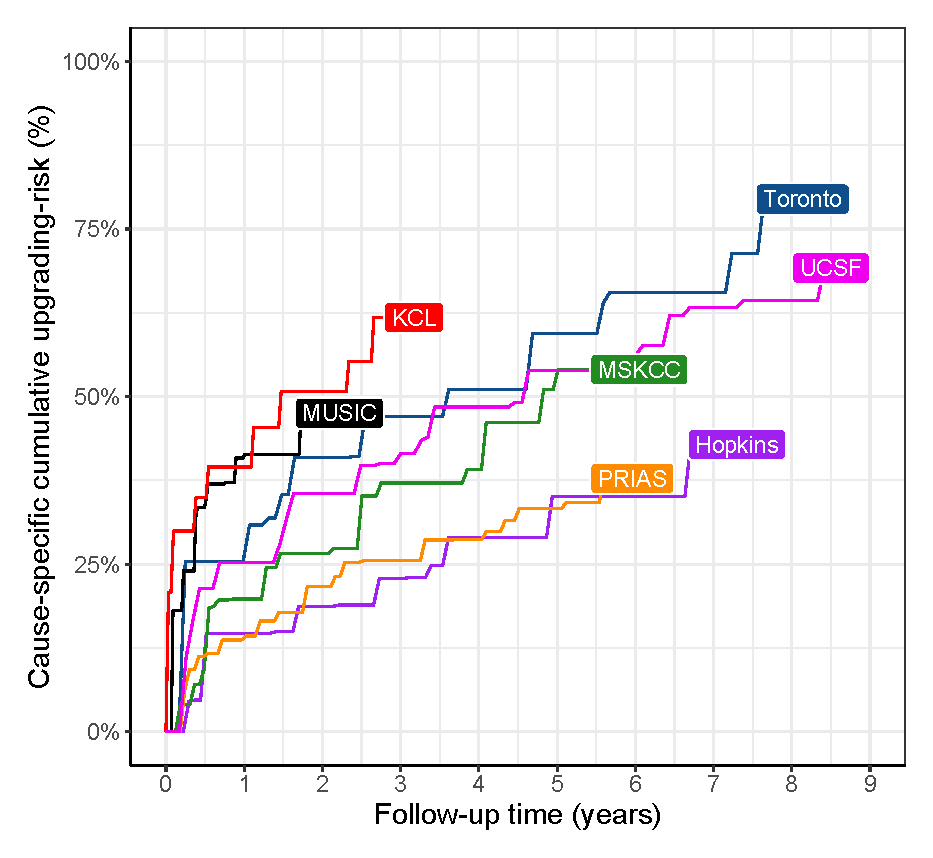
\includegraphics[width=\columnwidth]{images/npmle_plot.eps}}
\caption{\textbf{Nonparametric estimate \citep{turnbull1976empirical} of the cause-specific cumulative upgrading-risk} in the world's largest AS cohort PRIAS, and largest six AS cohorts from the GAP3 database \citep{gap3_2018}. Abbreviations are \textit{Hopkins}: Johns Hopkins Active Surveillance, \textit{PRIAS}: Prostate Cancer International Active Surveillance, \textit{Toronto}: University of Toronto Active Surveillance, \textit{MSKCC}: Memorial Sloan Kettering Cancer Center Active Surveillance, \textit{KCL}: King's College London Active Surveillance, \textit{MUSIC}: Michigan Urological Surgery Improvement Collaborative AS, \textit{UCSF}: University of California San Francisco Active Surveillance.}
\label{fig:npmle_plot}
\end{figure}

%\begin{landscape}
%\begin{table}
%\small\sf\centering
%\caption{\textbf{Summary of the five validation cohorts from the GAP3 database~\citep{gap3_2018}}. The primary event of interest is upgrading, that is, increase in Gleason grade group from group~1 to 2 or higher. \#PSA: number of PSA, \#biopsies: number of biopsies, IQR:~interquartile range, PSA:~prostate-specific antigen. Full names of cohorts are \textit{Hopkins}: Johns Hopkins Active Surveillance, \textit{PRIAS}: Prostate Cancer International Active Surveillance, \textit{Toronto}: University of Toronto Active Surveillance, \textit{MSKCC}: Memorial Sloan Kettering Cancer Center Active Surveillance, \textit{KCL}: King's College London Active Surveillance, \textit{MUSIC}: Michigan Urological Surgery Improvement Collaborative AS.}
%\label{table:gap3_summary}
%\begin{tabular}{lrrrrr}
%\hline
%\textbf{Characteristic} & \textbf{Hopkins} & \textbf{Toronto} & \textbf{MSKCC} & \textbf{MUSIC} & \textbf{KCL}\\
%\hline
%Total patients & 1392 & 1046 & 894 &  2743 & 616\\
%Upgrading (primary event) & 260 & 359 & 242 & 385 & 198\\
%\hline
%Median age (years) & 62 (IQR: 66--69) & 67 (IQR: 60--72) & 63 (IQR: 57--68) & 65 (IQR: 60--71) & 63 (IQR: 58--68)\\
%Median maximum follow-up per patient (years) &  3 (IQR: 1.3--5.8) & 4.5 (IQR: 1.9--8.4) & 5.3 (IQR: 1.8--8.3) & 1.2 (IQR: 0.6--2.2) & 2.4 (IQR: 1.3--3.8)\\
%Total PSA measurements & 11126 & 13984 & 10704 & 12087 & 2987\\
%Median \#PSA per patient &  6 (IQR: 4--11) & 12 (IQR: 7--19) & 11 (IQR: 5--17) & 4 (IQR: 2--6) & 4 (IQR: 2--6)\\
%Median PSA (ng/mL) & 4.7 (IQR: 2.9--6.7) & 6 (IQR: 3.7--9.0) & 4.7 (IQR: 2.8--7.1) & 5.1 (IQR: 3.4--7.1) & 6 (IQR: 4--9)\\
%Total biopsies & 1926 & 909 & 1102 & 1032 & 484\\
%Median \#biopsies per patient &  1 (IQR: 1--2) &  1 (IQR: 1--2) &  1 (IQR: 1--2) & 1 (IQR: 1--1) & 1 (IQR: 1--1)\\
%\hline
%\end{tabular}
%\end{table}
%\end{landscape}

\begin{table}
\small\sf\centering
\caption{\textbf{Summary of the Hopkins and Toronto validation cohorts from the GAP3 database~\citep{gap3_2018}}. The primary event of interest is upgrading, that is, increase in Gleason grade group from group~1 to 2 or higher. \#PSA: number of PSA, \#biopsies: number of biopsies, IQR:~interquartile range, PSA:~prostate-specific antigen. Full names of cohorts are \textit{Hopkins}: Johns Hopkins Active Surveillance, \textit{Toronto}: University of Toronto Active Surveillance}
\label{table:gap3_summary_1}
\begin{tabular}{lrr}
\hline
\textbf{Characteristic} & \textbf{Hopkins} & \textbf{Toronto}\\
\hline
Total patients & 1392 & 1046\\
Upgrading (primary event) & 260 & 359\\
\hline
Median age (years) & 62 (IQR: 66--69) & 67 (IQR: 60--72)\\
Median maximum follow-up per patient (years) &  3 (IQR: 1.3--5.8) & 4.5 (IQR: 1.9--8.4)\\
Total PSA measurements & 11126 & 13984\\
Median \#PSA per patient &  6 (IQR: 4--11) & 12 (IQR: 7--19)\\
Median PSA (ng/mL) & 4.7 (IQR: 2.9--6.7) & 6 (IQR: 3.7--9.0)\\
Total biopsies & 1926 & 909\\
Median \#biopsies per patient &  1 (IQR: 1--2) &  1 (IQR: 1--2)\\
\hline
\end{tabular}
\end{table}

\begin{table}
\small\sf\centering
\caption{\textbf{Summary of the MSKCC and UCSF validation cohorts from the GAP3 database~\citep{gap3_2018}}. The primary event of interest is upgrading, that is, increase in Gleason grade group from group~1 to 2 or higher. \#PSA: number of PSA, \#biopsies: number of biopsies, IQR:~interquartile range, PSA:~prostate-specific antigen. Full names of cohorts are \textit{MSKCC}: Memorial Sloan Kettering Cancer Center Active Surveillance, \textit{UCSF}: University of California San Francisco Active Surveillance.}
\label{table:gap3_summary_2}
\begin{tabular}{lrr}
\hline
\textbf{Characteristic} & \textbf{MSKCC} & \textbf{UCSF}\\
\hline
Total patients & 894 & 1397 \\
Upgrading (primary event) & 242 & 547\\
\hline
Median age (years) & 63 (IQR: 57--68) & 63 (IQR: 57--68)\\
Median maximum follow-up per patient (years) & 5.3 (IQR: 1.8--8.3) & 3.6 (IQR: 1.5--7.2)\\
Total PSA measurements & 10704 & 16093\\
Median \#PSA per patient & 11 (IQR: 5--17) & 8 (IQR: 4--16)\\
Median PSA (ng/mL) & 4.7 (IQR: 2.8--7.1) & 5.0 (IQR: 3.4--7.2)\\
Total biopsies & 1102 & 3512\\
Median \#biopsies per patient & 1 (IQR: 1--2) & 2 (IQR: 2--3)\\
\hline
\end{tabular}
\end{table}

\begin{table}
\small\sf\centering
\caption{\textbf{Summary of the MUSIC and KCL validation cohorts from the GAP3 database~\citep{gap3_2018}}. The primary event of interest is upgrading, that is, increase in Gleason grade group from group~1 to 2 or higher. \#PSA: number of PSA, \#biopsies: number of biopsies, IQR:~interquartile range, PSA:~prostate-specific antigen. Full names of cohorts are \textit{KCL}: King's College London Active Surveillance, \textit{MUSIC}: Michigan Urological Surgery Improvement Collaborative AS.}
\label{table:gap3_summary_3}
\begin{tabular}{lrr}
\hline
\textbf{Characteristic} & \textbf{MUSIC} & \textbf{KCL}\\
\hline
Total patients & 2743 & 616\\
Upgrading (primary event) & 385 & 198\\
\hline
Median age (years) & 65 (IQR: 60--71) & 63 (IQR: 58--68)\\
Median maximum follow-up per patient (years) & 1.2 (IQR: 0.6--2.2) & 2.4 (IQR: 1.3--3.8)\\
Total PSA measurements & 12087 & 2987\\
Median \#PSA per patient & 4 (IQR: 2--6) & 4 (IQR: 2--6)\\
Median PSA (ng/mL) & 5.1 (IQR: 3.4--7.1) & 6 (IQR: 4--9)\\
Total biopsies & 1032 & 484\\
Median \#biopsies per patient & 1 (IQR: 1--1) & 1 (IQR: 1--1)\\
\hline
\end{tabular}
\end{table}

The joint model was fitted using the R package \textbf{JMbayes} \citep{rizopoulosJMbayes}. This package utilizes the Bayesian methodology to estimate model parameters. The corresponding posterior parameter estimates are shown in Table~\ref{tab:PSA_long} (longitudinal sub-model for PSA outcome) and Table~\ref{tab:PSA_survival} (relative risk sub-model). The parameter estimates for the variance-covariance matrix $\boldsymbol{W}$ from the longitudinal sub-model for PSA are shown in the following Table~\ref{tab:D_matrix}:
\begin{table}
\small\sf\centering
\caption{\textbf{Estimated variance-covariance matrix} $\boldsymbol{W}$ of the random effects ${\boldsymbol{b}=(b_{0}, b_{1}, b_{2}, b_{3}, b_{4})}$ from the joint model fitted to the PRIAS dataset. The variances of the random effects are highlighted along the diagonal of the variance-covariance matrix.}
\label{tab:D_matrix}
\begin{tabular}{lrrrrr}
\hline
Random Effects    & $b_{0}$    & $b_{1}$   & $b_{2}$   & $b_{3}$   & $b_{4}$    \\
\hline
$b_{0}$ & \textbf{0.229} & 0.030 & 0.023 & 0.073 & 0.007 \\
$b_{1}$ & 0.030 & \textbf{0.149} & 0.098 & 0.171 & 0.085 \\
$b_{2}$ & 0.023 & 0.098 & \textbf{0.276} & 0.335 & 0.236 \\
$b_{3}$ & 0.073 & 0.171 & 0.335 & \textbf{0.560} & 0.359 \\
$b_{4}$ & 0.007 & 0.085 & 0.236 & 0.359 & \textbf{0.351} \\
\hline
\end{tabular}
\end{table}

For the PSA mixed effects sub-model parameter estimates (see Equation \ref{eq:long_model_psa}), in Table~\ref{tab:PSA_long} we can see that the age of the patient trivially affects the baseline ${\log_2(\mbox{PSA} + 1)}$ measurement. Since the longitudinal evolution of ${\log_2 (\mbox{PSA} + 1)}$ measurements is modeled with non-linear terms, the interpretation of the coefficients corresponding to time is not straightforward. In lieu of the interpretation, in Figure~\ref{fig:fitted_9subject_psa} we present plots of observed versus fitted PSA profiles for nine randomly selected patients. 
\begin{table}
\small\sf\centering
\caption{\textbf{Parameters of the longitudinal sub-model}: Estimated mean and 95\% credible interval for parameters in Equation (\ref{eq:long_model_psa}).}
\label{tab:PSA_long}
\begin{tabular}{lrrrrr}
\hline
Variable                         & Mean & Std. Dev & 2.5\%  & 97.5\% & P     \\
\hline
Intercept & 2.129    & 0.060  & 2.009 & 2.244 & \textless0.001 \\
Age & 0.008    & 0.001 & 0.007 & 0.010   &\textless0.001 \\
Spline: [0.0, 0.5] years & 0.063    & 0.007 & 0.051 & 0.075  & \textless0.001 \\
Spline: [0.5, 1.3] years & 0.196    & 0.010  & 0.177 & 0.217  & \textless0.001 \\
Spline: [1.3, 3.0] years & 0.244    & 0.014 & 0.217 & 0.272  & \textless0.001 \\
Spline: [3.0, 6.3] years & 0.382    & 0.014 & 0.356 & 0.410 &  \textless0.001 \\
$\sigma$ & 0.139    & 0.001 & 0.138 & 0.140  & \\
\hline
\end{tabular}
\end{table}

\begin{figure}
\centerline{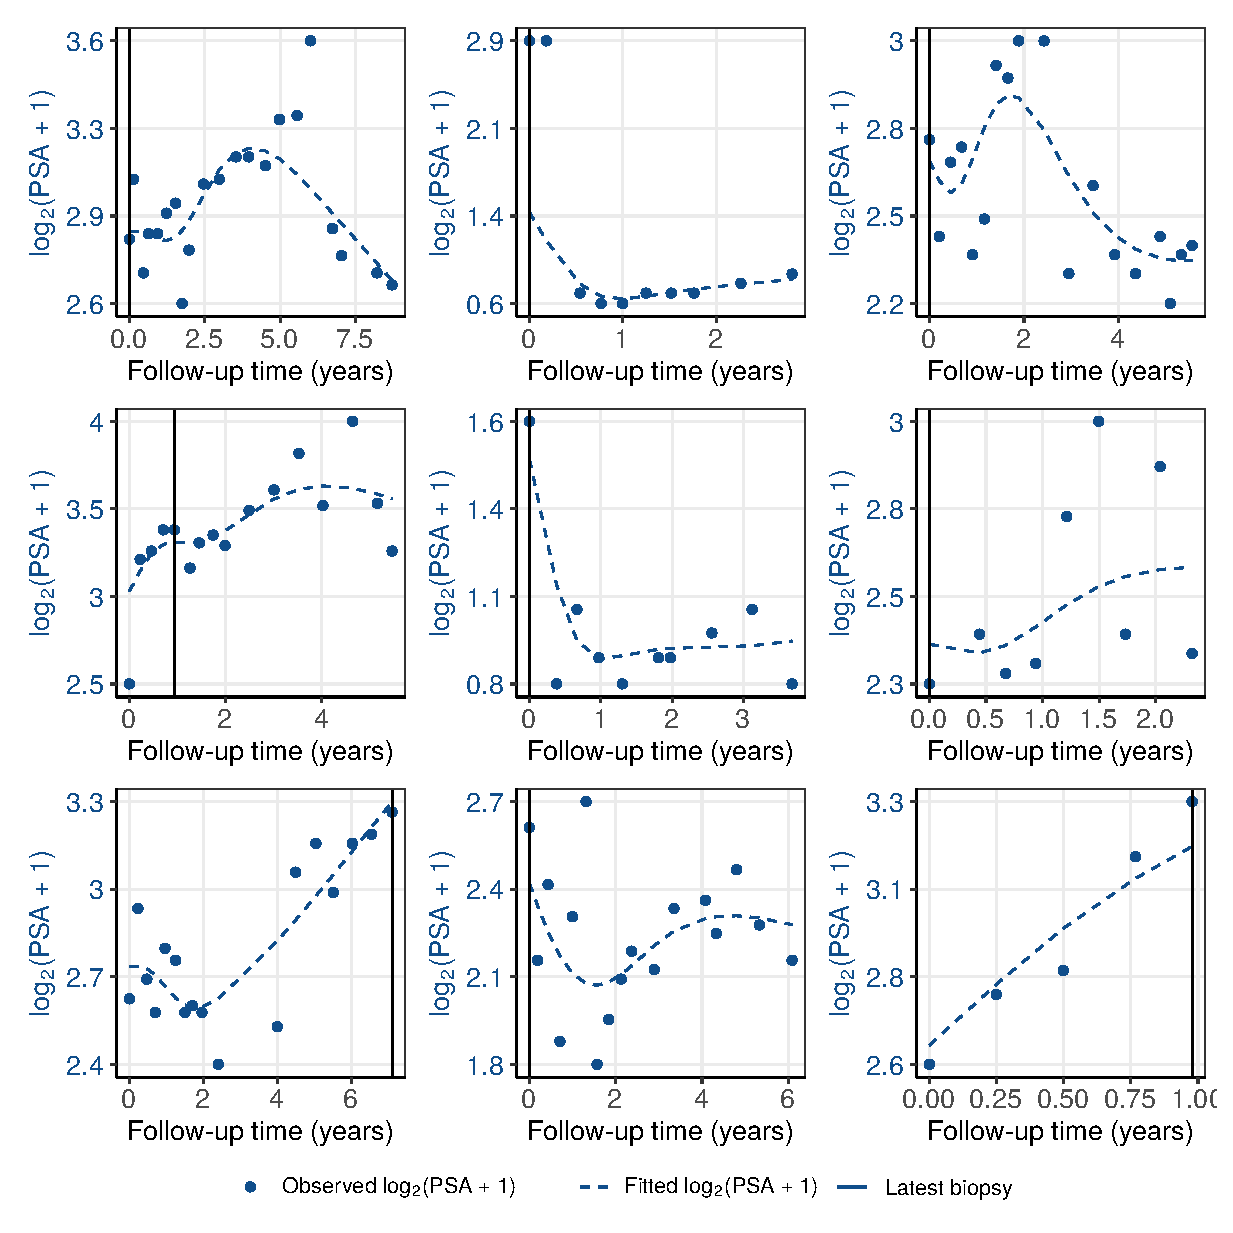
\includegraphics[width=\columnwidth]{images/fitted_9subject_psa.eps}}
\caption{\textbf{Fitted versus observed ${\log_2 (\mbox{PSA} + 1)}$ profiles} for nine randomly selected PRIAS patients. The fitted profiles utilize information from the observed PSA measurements, and time of the latest biopsy.}
\label{fig:fitted_9subject_psa}
\end{figure}

For the relative risk sub-model (see Equation \ref{eq:rel_risk_model}), the parameter estimates in Table~\ref{tab:PSA_survival} show that ${\log_2 (\mbox{PSA} + 1)}$ velocity and age of the patient were significantly associated with the hazard of upgrading.

\begin{table}
\small\sf\centering
\caption{\textbf{Parameters of the relative risk sub-model}: Estimated mean and 95\% credible interval for the parameters in Equation (\ref{eq:rel_risk_model}).}
\label{tab:PSA_survival}
\begin{tabular}{lrrrrr}
\hline
Variable                      & Mean   & Std. Dev & 2.5\%  & 97.5\%                 & P              \\
\hline
Age                      & 0.037    & 0.006 & 0.025  & 0.049  & \textless0.001 \\
Fitted $\log_2 (\mbox{PSA} + 1)$ value            & -0.012   & 0.076 & -0.164 & 0.135  & 0.856 \\
Fitted $\log_2 (\mbox{PSA} + 1)$ velocity             & 2.266    & 0.299 & 1.613  & 2.767  & \textless0.001   \\
\hline
\end{tabular}
\end{table}

It is important to note that since age, and ${\log_2 (\mbox{PSA} + 1)}$ value and velocity are all measured on different scales, a comparison between the corresponding parameter estimates is not easy. To this end, in Table \ref{tab:PSA_survival_easy}, we present the hazard ratio of upgrading, for an increase in the aforementioned variables from their 25-th to the 75-th percentile. For example, an increase in fitted $\log_2 (\mbox{PSA} + 1)$ velocity from -0.085 to 0.308 (fitted 25-th and 75-th percentiles) corresponds to a hazard ratio of 2.433. The interpretation of the rest is similar.

\begin{table}
\small\sf\centering
\caption{\textbf{Hazard ratio and 95\% credible interval (CI) for upgrading}: Variables are on different scale and hence we compare an increase in the variables of relative risk sub-model from their 25-th percentile ($\mbox{P}_{25}$) to their 75-th percentile ($\mbox{P}_{75}$). Except for age, quartiles for all other variables are based on their fitted values obtained from the joint model fitted to the PRIAS dataset.}
\label{tab:PSA_survival_easy}
\begin{tabular}{lrrr}
\hline
Variable                      & $\mbox{P}_{25}$   & $\mbox{P}_{75}$ & Hazard ratio [95\% CI] \\
\hline
Age & 61 & 71 & 1.455 [1.285, 1.631] \\
Fitted $\log_2 (\mbox{PSA} + 1)$ value & 2.360 & 3.078 & 0.991 [0.889, 1.102] \\
Fitted $\log_2 (\mbox{PSA} + 1)$ velocity & -0.085 & 0.308 & 2.433 [1.883, 2.962] \\
\hline
\end{tabular}
\end{table}

\begin{table}
\small\sf\centering
\caption{\textbf{Parameters of the relative risk sub-model in validation cohorts}. We fitted separate joint models for each of the six GAP3 validation cohorts as well. The specification of these joint models was same as that of the model for PRIAS. Two important predictors in the relative-risk sub-model, namely, the $\log_2 (\mbox{PSA} + 1)$ value and velocity have different impact on upgrading-risk across the cohorts. Table shows the mean estimate of these parameters with 95\% credible interval in brackets. Strongest average effect of $\log_2 (\mbox{PSA} + 1)$ velocity is in PRIAS cohort, whereas the weakest is in MUSIC cohort. The strongest average effect of $\log_2 (\mbox{PSA} + 1)$ value is in the Toronto cohort whereas the weakest is in PRIAS cohort. Full names of cohorts are \textit{Hopkins}: Johns Hopkins Active Surveillance, \textit{PRIAS}: Prostate Cancer International Active Surveillance, \textit{Toronto}: University of Toronto Active Surveillance, \textit{MSKCC}: Memorial Sloan Kettering Cancer Center Active Surveillance, \textit{KCL}: King's College London Active Surveillance, \textit{MUSIC}: Michigan Urological Surgery Improvement Collaborative AS, \textit{UCSF}: University of California San Francisco Active Surveillance.}
\label{tab:PSA_survival_gap3}
\begin{tabular}{lrr}
\hline
Cohort & Fitted $\log_2 (\mbox{PSA} + 1)$ value & Fitted $\log_2 (\mbox{PSA} + 1)$ velocity\\
\hline
PRIAS & -0.012 [-0.164, 0.135] & 2.266 [ 1.613, 2.767]\\
Hopkins & 0.061 [-0.323, 0.329] & 1.839 [ 0.761, 4.378]\\
MSKCC & 0.336 [ 0.081, 0.583] & 1.122 [ 0.421, 1.980]\\
Toronto & 0.572 [ 0.347, 0.794] & 0.943 [ 0.464, 1.554]\\
UCSF & 0.498 [ 0.326, 0.673] & 0.812 [ 0.280, 1.383]\\
MUSIC & 0.441 [ 0.092, 0.767] & 0.029 [-0.552, 0.512]\\
KCL &  0.194 [-0.104, 0.540] & 0.840 [-0.087, 1.665]\\
\hline
\end{tabular}
\end{table}